\documentclass[a0,landscape]{a0poster}

\renewcommand{\familydefault}{\sfdefault}

\usepackage{multicol} % This is so we can have multiple columns of text side-by-side
\columnsep=100pt % This is the amount of white space between the columns in the poster
\columnseprule=3pt % This is the thickness of the black line between the columns in the poster

\usepackage[svgnames]{xcolor} % Specify colors by their 'svgnames', for a full list of all colors available see here: http://www.latextemplates.com/svgnames-colors

%\usepackage{times} % Use the times font
%\usepackage{palatino} % Uncomment to use the Palatino font

\usepackage{graphicx} % Required for including images

\graphicspath{{images/}} % Location of the graphics files

\usepackage{booktabs} % Top and bottom rules for table

\usepackage[font=small,labelfont=bf]{caption} % Required for specifying captions to tables and figures

\usepackage{amsfonts, amsmath, amsthm, amssymb} % For math fonts, symbols and environments

\usepackage{wrapfig} % Allows wrapping text around tables and figures

\usepackage{url}

\usepackage{minted}
\newminted{julia}{breaklines}

\begin{document}

%----------------------------------------------------------------------------------------
%	POSTER HEADER 
%----------------------------------------------------------------------------------------

% The header is divided into three boxes:
% The first is 55% wide and houses the title, subtitle, names and university/organization
% The second is 25% wide and houses contact information
% The third is 19% wide and houses a logo for your university/organization or a photo of you
% The widths of these boxes can be easily edited to accommodate your content as you see fit

\begin{minipage}[b]{0.60\linewidth}
{\Huge \color{NavyBlue} \textbf{\texttt{PWDFT.jl}: A Julia package for electronic structure calculation \\
using density functional theory and plane wave basis} \color{Black}}\\
\huge \textbf{Fadjar Fathurrahman, Muhammad Kemal Agusta \& Hermawan Kresno Dipojono }\\ % Author(s)
\huge Kelompok Keahlian Teknik Fisika Institut Teknologi Bandung \\ % University/organization
\end{minipage}
%
\begin{minipage}[b]{0.15\linewidth}
\color{DarkSlateGray}\Large \textbf{Contact Information:}\\
Kelompok Keahlian Teknik Fisika \\ % Address
Institut Teknologi Bandung \\
Email: \texttt{fadjar@tf.itb.ac.id}\\ % Email address
\end{minipage}
%
\begin{minipage}[b]{0.125\linewidth}

\includegraphics[width=10cm]{ITB_logo.pdf}\\
\end{minipage}
%
\begin{minipage}[b]{0.125\linewidth}

\includegraphics[width=10cm]{julia-logo-circular.pdf}\\
\end{minipage}

\vspace{1cm} % A bit of extra whitespace between the header and poster content

%----------------------------------------------------------------------------------------

\begin{multicols}{3}

%----------------------------------------------------------------------------------------
%	ABSTRACT
%----------------------------------------------------------------------------------------

\color{Navy} % Navy color for the abstract

\begin{minipage}[b]{1.0\linewidth}
\Large

{\centering \textbf{ABSTRACT} \par}

We describe the implementation of \texttt{PWDFT.jl}, a package for electronic
structure calculations written using Julia programming language using
plane wave basis set and pseudopotentials.
In this package, typical Kohn-Sham density functional theory (KSDFT) is divided into three
steps: instantiation of an atomistic models, initialization of Kohn-Sham
Hamiltonian, and self-consistent field (SCF) calculations.
\texttt{PWDFT.jl} is allows user to write their own SCF or alternative methods
by providing implementation several basic operations such as wave function
orthogonalization, action of kinetic and potential operators
to wave functions and iterative diagonalization
of Hamiltonian. Because \texttt{PWDFT.jl} is implemented in Julia, matrix operations
within which plane wave KSDFT are formulated, are particularly easy to be implemented
as used.
With these features\texttt{PWDFT.jl} is expected to be useful for for beginners KSDFT
implementers and researchers who want to implement their new methods quickly.
\texttt{PWDFT.jl} is freely available at
\url{https:/github.com/f-fathurrahman/PWDFT.jl}.
\end{minipage}



%----------------------------------------------------------------------------------------
%	INTRODUCTION
%----------------------------------------------------------------------------------------

\color{SaddleBrown} % SaddleBrown color for the introduction


\section*{Introduction}

Electronic structure calculations based on Kohn-Sham density functional theory (KSDFT)
\cite{Hohenberg1964,Kohn1965} is very popular nowadays.
It is routinely used to model and predict various materials properties
\cite{Martin2004} by researchers from various fields
such as physics, chemistry, and engineering.
In practice, KSDFT calculations typically are carried out by using
program packages such as Quantum Espresso \cite{Giannozzi2009},
VASP \cite{Kresse1996a}, and
ABINIT \cite{Gonze2009}.
While using such program packages are very convenient for most practical
purposes\, these packages arguably
is not ideal for development.
One factor which make development difficult for those program packages is
due to the fact that they are written using static programming
languages such Fortran and C/C++.
Several attempts has been made to make development easy by using
dynamic programming languages such as Python (GPAW package \cite{Enkovaara2010})
and MATLAB (KSSOLV package \cite{Yang2009}).
However, the speed of execution of dynamic programming languages is generally
slower than static programming language, so in order to obtain good performance
one need to implement the time-consuming part of the code in C or Fortran which
can hinder development of the code because programmers need to deal with
low level details such as manual memory management.



\color{DarkSlateGray} % DarkSlateGray color for the rest of the content

\section*{Main Objectives}

The main objective of this research is to
implement a software package for doing Kohn-Sham density functional
calculations with plane wave basis set and pseudopotentials.
This software package should be simple yet able to carry out
total energy calculations for non-trivial systems (not only toy
models used in textbook).

\section*{Proposed solution}

In this research we implement a software package named \texttt{PWDFT.jl}
to carry out plane wave density functional calculations. This package
is written in Julia programming language. Julia is a high-level dynamic
programming language which has similarities to other dynamic languages
such as MATLAB, R and Python. As opposed to those dynamics language, Julia
can achieve near-C-performance without having to write some portion of the
code in C or Fortran. Julia also has first class support of multidimensional
arrays like MATLAB which facilitates rapid development and quick prototyping
for new algorithms.

\section*{Basic theory}

In KSDFT approach \cite{Hohenberg1964,Kohn1965}, total energy per unit cell system
$E^{\mathrm{KS}}_{\mathrm{total}}$ can be written as
\begin{equation}
E^{\mathrm{KS}}_{\mathrm{total}} =
E_{\mathrm{kin}} + E_{\mathrm{ele-nuc}} +
E_{\mathrm{Ha}} + E_{\mathrm{xc}} + E_{\mathrm{nuc-nuc}}
\label{eq:E_KS_total}
\end{equation}
with $E_\mathrm{kin}$ is the non-interacting kinetic energy of electrons,
$E_{\mathrm{ele-nuc}}$ is the interaction energy between electrons and nuclei,
$E_{\mathrm{Ha}}$ is the classical electrostatic or Hartree energy,
$E_{\mathrm{xc}}$ is the exchange-correlation energy, and
$E_{\mathrm{nuc-nuc}}$ is the interaction energy between nuclei.
Central to the Kohn-Sham DFT is the one-electron
(Kohn-Sham) orbitals $\psi_{i,\mathbf{k}}(\mathbf{r})$
with the associated orbital energies $\epsilon_{i,\mathbf{k}}$
and the electron density $\rho(\mathbf{r})$ which is obtained from
the Kohn-Sham orbitals
\begin{equation}
\rho(\mathbf{r}) = \sum_{\mathbf{k}} 
\sum_{i=1}^{N_{\mathbf{occ}}}
w_{\mathbf{k}}
f_{i,\mathbf{k}}
\psi^{*}_{i,\mathbf{k}}(\mathbf{r})
\psi_{i,\mathbf{k}}(\mathbf{r})
\label{eq:rhoel}
\end{equation}
%
\begin{equation}
\psi_{i,\mathbf{k}}(\mathbf{r}) = 
\frac{1}{\sqrt{\Omega}}
\sum_{\mathbf{G}}
c_{i,\mathbf{G}+\mathbf{k}}
\exp\left[
\mathrm{i}\left(\mathbf{G}+\mathbf{k}\right)\cdot\mathbf{r}
\right]
\end{equation}
%
\begin{equation}
E_{\mathrm{kin}} = -\frac{1}{2} \sum_{\mathbf{k}} \sum_{i}
w_{\mathbf{k}} f_{i,\mathbf{k}}
\int_{\Omega}
\psi^{*}_{i,\mathbf{k}}(\mathbf{r})
\nabla^2
\psi_{i,\mathbf{k}}(\mathbf{r})
\,
\mathrm{d}\mathbf{r}
\label{eq:Kin_energy}
\end{equation}
%
\begin{equation}
E_{\mathrm{ele-nuc}} = 
\sum_{\mathbf{k}}
\sum_{i}
w_{\mathbf{k}}
f_{i,\mathbf{k}}
\int_{\Omega}\,
\psi^{*}_{i,\mathbf{k}}(\mathbf{r})
V_{\mathrm{ele-nuc}}(\mathbf{r})
\psi_{i,\mathbf{k}}(\mathbf{r})
\,\mathrm{d}\mathbf{r}.
\label{eq:E_ele_nuc}
\end{equation}
%
\begin{equation}
E_{\mathrm{Ha}} = \frac{1}{2}
\int_{\Omega}
V_{\mathrm{Ha}}(\mathbf{r})\rho(\mathbf{r})\,
\mathrm{d}\mathbf{r}
\end{equation}
%
\begin{equation}
V_{\mathrm{Ha}}(\mathbf{r}) =
\int_{\Omega}
\frac{\rho(\mathbf{r}')}{\mathbf{r} - \mathbf{r}'}
\,\mathrm{d}\mathbf{r}'
\end{equation}
%
\begin{equation}
\nabla^2 V_{\mathrm{Ha}}(\mathbf{r}) =
-4\pi\rho(\mathbf{r})
\end{equation}
%
\begin{equation}
E_{\mathrm{xc}} = 
\int_{\Omega}
\rho(\mathbf{r})
\epsilon_{\mathrm{xc}}\left[\rho(\mathbf{r})\right]
\,\mathrm{d}\mathbf{r}
\end{equation}
%
\begin{equation}
E_{\mathrm{nuc-nuc}} =
\frac{1}{2}
\sum_{I \neq J} Z_{I} Z_{J} \left[
\frac{\mathrm{erfc}\left( \eta
\left| \mathbf{R}_{I} - \mathbf{R}_{J} - \mathbf{T} \right|
\right)}
{\left| \mathbf{R}_{I} - \mathbf{R}_{J} - \mathbf{T} \right|}
+
\frac{4\pi}{\Omega} \sum_{\mathbf{G}\neq \mathbf{0}}
\frac{1}{G^2} \exp\left(-\dfrac{G^2}{4\eta^2}\right)
\cos\left(\mathbf{G}\cdot(\mathbf{R}_{I} - \mathbf{R}_{J})\right)
\right]
\end{equation}


%----------------------------------------------------------------------------------------
%	RESULTS 
%----------------------------------------------------------------------------------------

\section*{Results}

The program package can be obtained from the Github repository at:
\url{https://github.com/f-fathurrahman/PWDFT.jl}

\begin{center}
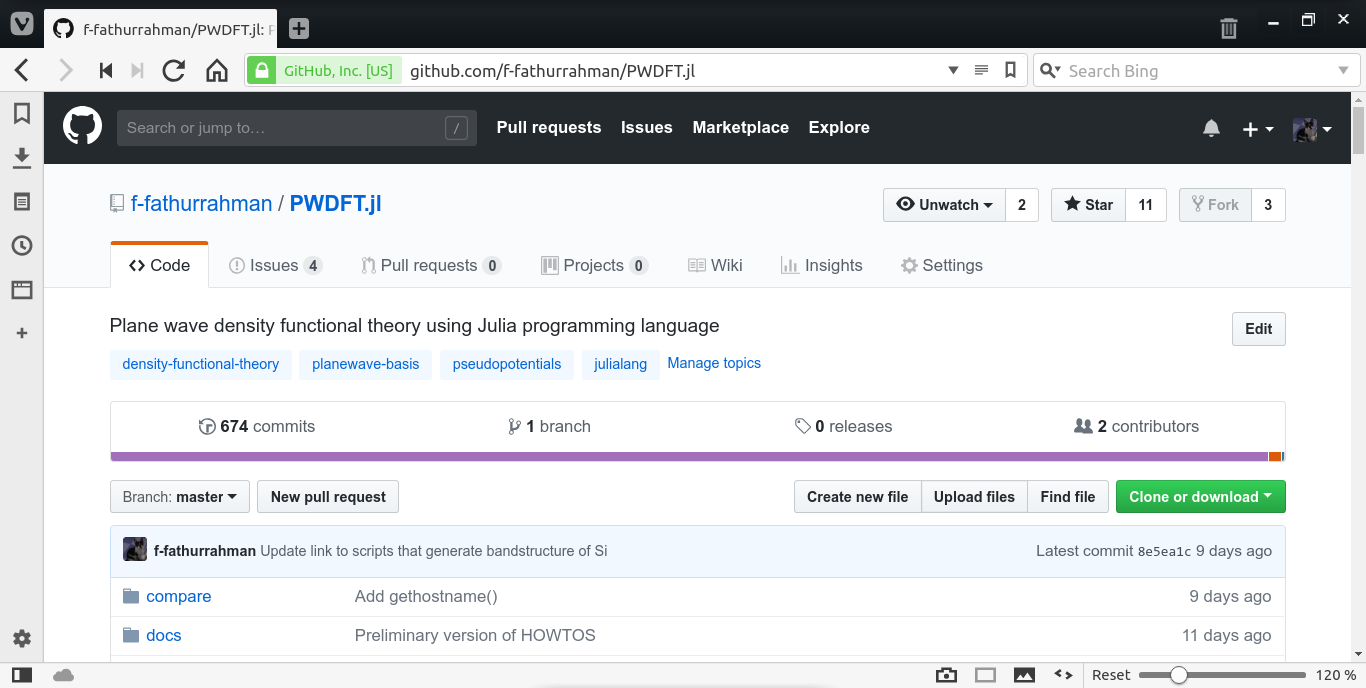
\includegraphics[width=0.8\linewidth]{PWDFT_github.png}
\captionof{figure}{\color{Green} Github repository of \texttt{PWDFT.jl}}
\end{center}

The following code shows how one can calculate total energy of a molecule
defined in an xyz file:

\begin{juliacode}
# Load the package
using PWDFT
# Stage 1: Initialization of atomic structures
atoms = Atoms(xyz_file="CH4.xyz")
# Stage 2: Initialization of Hamiltonian
ecutwfc = 15.0  # cutoff energy in hartree
pspfiles = ["C-q4.gth", "H-q1.gth"] # path to pseudopotential files
Ham = Hamiltonian( atoms, pspfiles, ecutwfc )
# Stage 3: Solve the Kohn-Sham problem
KS_solve_SCF!( Ham, betamix=0.2 )
\end{juliacode}

Using \texttt{PWDFT.jl} one also can obtain various numerical data
and processes it for visualization or other analysis. As an example,
in Figure \ref{fig:HCobalt4CO} highest occupied molecular orbitals
of cobalt hydrocarbonyl $\textrm{HCo(CO)}_{4}$ is visualized.

\begin{center}
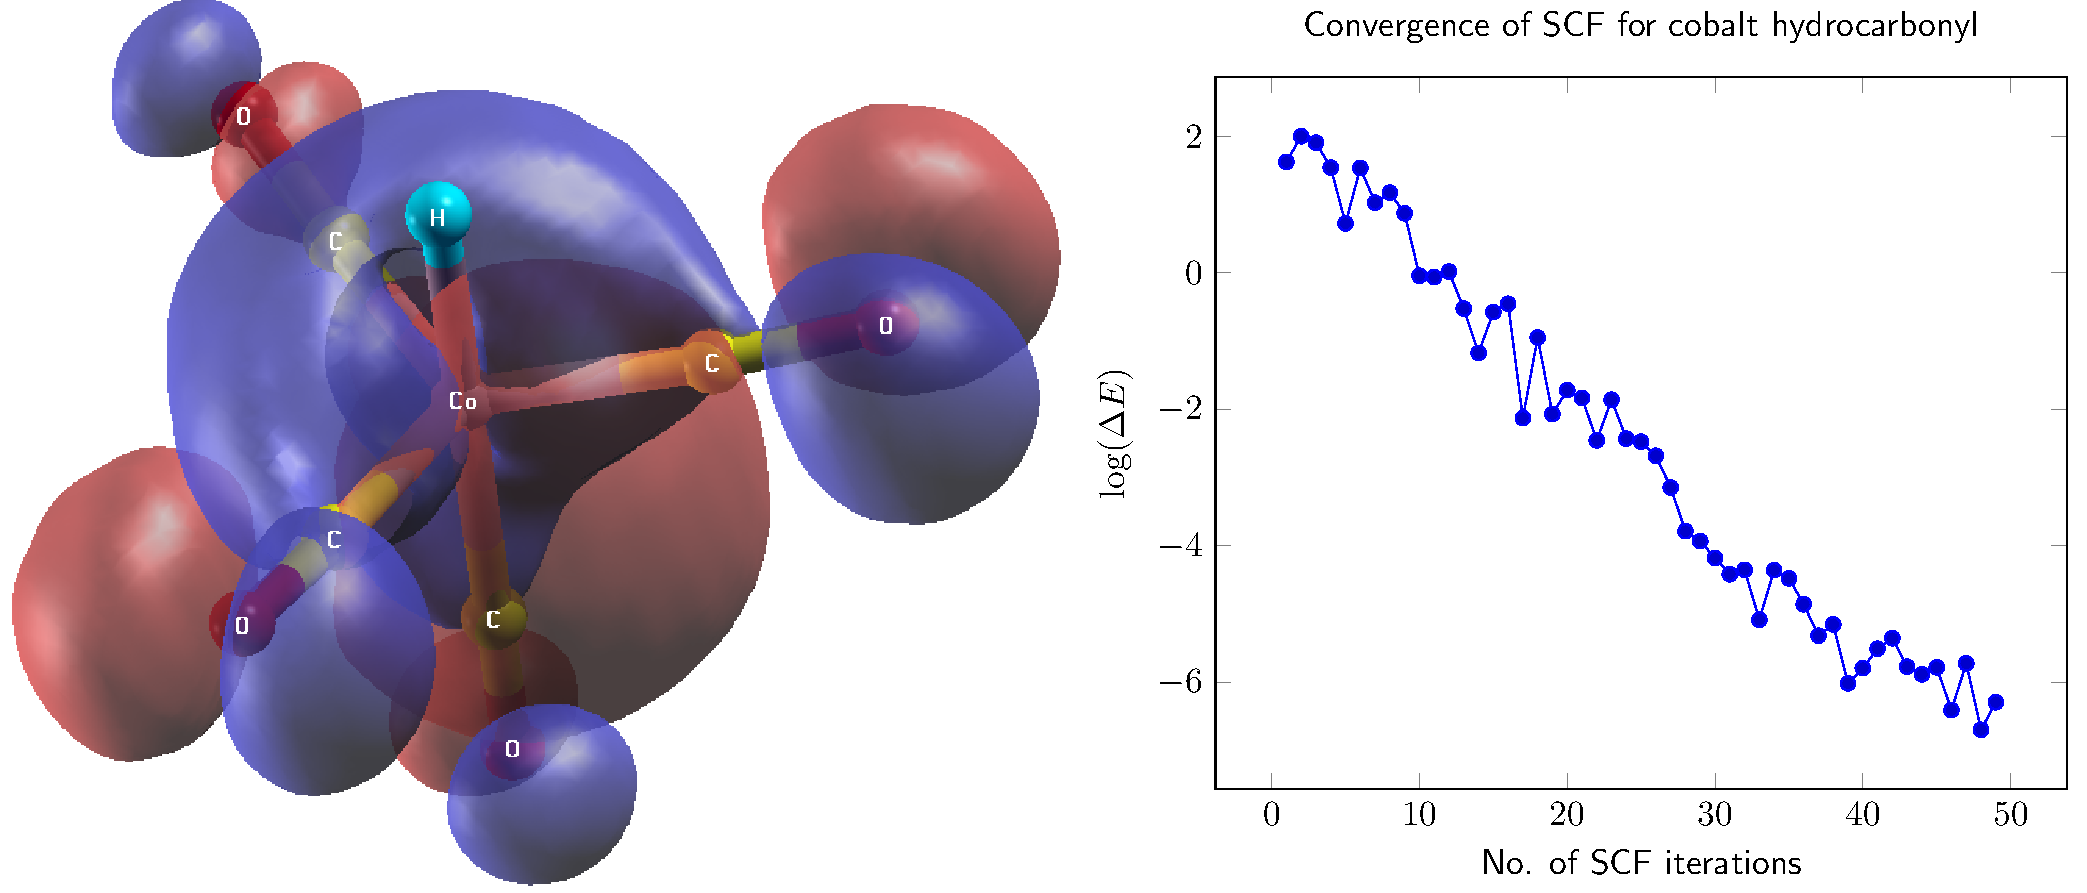
\includegraphics[scale=1.0]{figure02.pdf}
\captionof{figure}{\color{Green} Highest molecular orbital of cobalt hydrocarbonyl
(left) and progress of its SCF convergence (right)}
\label{fig:HCobalt4CO}
\end{center}



\color{SaddleBrown} % SaddleBrown color for the conclusions to make them stand out

\section*{Conclusions}

\begin{itemize}
\item Pellentesque eget orci eros. Fusce ultricies, tellus et pellentesque fringilla, ante massa luctus libero, quis tristique purus urna nec nibh. Phasellus fermentum rutrum elementum. Nam quis justo lectus.
\item Vestibulum sem ante, hendrerit a gravida ac, blandit quis magna.
\item Donec sem metus, facilisis at condimentum eget, vehicula ut massa. Morbi consequat, diam sed convallis tincidunt, arcu nunc.
\item Nunc at convallis urna. isus ante. Pellentesque condimentum dui. Etiam sagittis purus non tellus tempor volutpat. Donec et dui non massa tristique adipiscing.
\end{itemize}

\color{DarkSlateGray} % Set the color back to DarkSlateGray for the rest of the content

\section*{Forthcoming Research}

\begin{itemize}
\item Parallelization using MPI and CUDA
\item Direct minimization algorithm for metallic systems
\end{itemize}

%\bibliographystyle{plain} % Plain referencing style
%\bibliography{BIBLIO} % Use the example bibliography file sample.bib

\begin{thebibliography}{0}
\bibitem{Hohenberg1964} P. Hohenberg and W. Kohn. \textit{Phys. Rev.} \textbf{136}
 (1964) B864–871.
\bibitem{Kohn1965} W. Kohn and L. Sham. \textit{Phys. Rev.} \textbf{140} (4A) (1965) A1333–1138.
\bibitem{Martin2004} R. Martin. \textit{Electronic Structure, Basic Theory and Practical Methods}, CUP, Cambridge, UK, 2004.
\bibitem{Giannozzi2009} P. Giannozzi, et al. \textit{J. Phys. Condens. Matt.}
\textbf{21} (2009) 395502.
\bibitem{Kresse1996a} G. Kresse and J. Furthmüller. \textit{Comp. Mat. Sci.}
\textbf{6} (1996) 15–50.
\bibitem{Gonze2009} X. Gonze, et al. \textit{Comp. Phys. Comm.} \textbf{180}
(2009) 2582-2615.
\bibitem{Enkovaara2010} J. Enkovaara, et al. \textit{J. Phys: Cond. Matt}
\textbf{22} (2010) 253202.
\bibitem{Yang2009} C. Yang, et al. \textit{ACM Trans. Math. Softw.}
\textbf{36} (2009) 10:1-10:35.
\end{thebibliography}


%\section*{Acknowledgements}



%----------------------------------------------------------------------------------------

\end{multicols}


\end{document}
